% Graphic for TeX using PGF
% Title: /home/afoek/Diagram1.dia
% Creator: Dia v0.97+git
% CreationDate: Wed Oct 28 11:34:55 2020
% For: afoek
% \usepackage{tikz}
% The following commands are not supported in PSTricks at present
% We define them conditionally, so when they are implemented,
% this pgf file will use them.
\ifx\du\undefined
  \newlength{\du}
\fi
\setlength{\du}{15\unitlength}
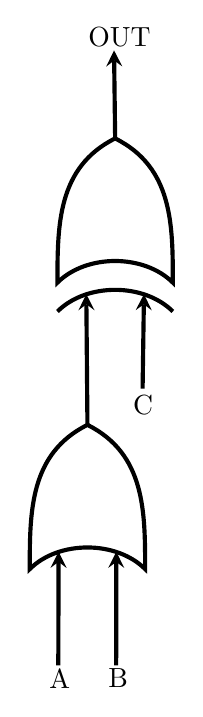
\begin{tikzpicture}[even odd rule]
\pgftransformxscale{1.000000}
\pgftransformyscale{-1.000000}
\definecolor{dialinecolor}{rgb}{0.000000, 0.000000, 0.000000}
\pgfsetstrokecolor{dialinecolor}
\pgfsetstrokeopacity{1.000000}
\definecolor{diafillcolor}{rgb}{1.000000, 1.000000, 1.000000}
\pgfsetfillcolor{diafillcolor}
\pgfsetfillopacity{1.000000}
\pgfsetlinewidth{0.100000\du}
\pgfsetdash{}{0pt}
\pgfsetbuttcap
\pgfsetmiterjoin
\pgfsetlinewidth{0.100000\du}
\pgfsetbuttcap
\pgfsetmiterjoin
\pgfsetdash{}{0pt}
\definecolor{diafillcolor}{rgb}{1.000000, 1.000000, 1.000000}
\pgfsetfillcolor{diafillcolor}
\pgfsetfillopacity{1.000000}
\definecolor{dialinecolor}{rgb}{0.000000, 0.000000, 0.000000}
\pgfsetstrokecolor{dialinecolor}
\pgfsetstrokeopacity{1.000000}
\pgfpathmoveto{\pgfpoint{-11.275178\du}{10.134061\du}}
\pgfpathcurveto{\pgfpoint{-9.885373\du}{10.828963\du}}{\pgfpoint{-9.885373\du}{12.218767\du}}{\pgfpoint{-9.885373\du}{13.608572\du}}
\pgfpathcurveto{\pgfpoint{-10.580276\du}{12.913670\du}}{\pgfpoint{-11.970080\du}{12.913670\du}}{\pgfpoint{-12.664982\du}{13.608572\du}}
\pgfpathcurveto{\pgfpoint{-12.664982\du}{12.218767\du}}{\pgfpoint{-12.664982\du}{10.828963\du}}{\pgfpoint{-11.275178\du}{10.134061\du}}
\pgfpathclose
\pgfusepath{fill,stroke}
\pgfsetlinewidth{0.010000\du}
\pgfsetbuttcap
\pgfsetmiterjoin
\pgfsetdash{}{0pt}
\definecolor{dialinecolor}{rgb}{0.000000, 0.000000, 0.000000}
\pgfsetstrokecolor{dialinecolor}
\pgfsetstrokeopacity{1.000000}
\pgfpathmoveto{\pgfpoint{-11.275178\du}{10.134061\du}}
\pgfpathcurveto{\pgfpoint{-9.885373\du}{10.828963\du}}{\pgfpoint{-9.885373\du}{12.218767\du}}{\pgfpoint{-9.885373\du}{13.608572\du}}
\pgfpathcurveto{\pgfpoint{-10.580276\du}{12.913670\du}}{\pgfpoint{-11.970080\du}{12.913670\du}}{\pgfpoint{-12.664982\du}{13.608572\du}}
\pgfpathcurveto{\pgfpoint{-12.664982\du}{12.218767\du}}{\pgfpoint{-12.664982\du}{10.828963\du}}{\pgfpoint{-11.275178\du}{10.134061\du}}
\pgfusepath{stroke}
\pgfsetlinewidth{0.100000\du}
\pgfsetdash{}{0pt}
\pgfsetbuttcap
{
\definecolor{diafillcolor}{rgb}{0.000000, 0.000000, 0.000000}
\pgfsetfillcolor{diafillcolor}
\pgfsetfillopacity{1.000000}
% was here!!!
\pgfsetarrowsend{stealth}
\definecolor{dialinecolor}{rgb}{0.000000, 0.000000, 0.000000}
\pgfsetstrokecolor{dialinecolor}
\pgfsetstrokeopacity{1.000000}
\draw (-11.977160\du,15.926808\du)--(-11.970080\du,13.191630\du);
}
\pgfsetlinewidth{0.100000\du}
\pgfsetdash{}{0pt}
\pgfsetbuttcap
{
\definecolor{diafillcolor}{rgb}{0.000000, 0.000000, 0.000000}
\pgfsetfillcolor{diafillcolor}
\pgfsetfillopacity{1.000000}
% was here!!!
\pgfsetarrowsend{stealth}
\definecolor{dialinecolor}{rgb}{0.000000, 0.000000, 0.000000}
\pgfsetstrokecolor{dialinecolor}
\pgfsetstrokeopacity{1.000000}
\draw (-10.583070\du,15.926808\du)--(-10.580276\du,13.191630\du);
}
\pgfsetlinewidth{0.100000\du}
\pgfsetdash{}{0pt}
\pgfsetbuttcap
{
\definecolor{diafillcolor}{rgb}{0.000000, 0.000000, 0.000000}
\pgfsetfillcolor{diafillcolor}
\pgfsetfillopacity{1.000000}
% was here!!!
\pgfsetarrowsend{stealth}
\definecolor{dialinecolor}{rgb}{0.000000, 0.000000, 0.000000}
\pgfsetstrokecolor{dialinecolor}
\pgfsetstrokeopacity{1.000000}
\draw (-11.275178\du,10.134061\du)--(-11.302628\du,6.985362\du);
}
\pgfsetlinewidth{0.100000\du}
\pgfsetdash{}{0pt}
\pgfsetbuttcap
\pgfsetmiterjoin
\pgfsetlinewidth{0.100000\du}
\pgfsetbuttcap
\pgfsetmiterjoin
\pgfsetdash{}{0pt}
\definecolor{diafillcolor}{rgb}{1.000000, 1.000000, 1.000000}
\pgfsetfillcolor{diafillcolor}
\pgfsetfillopacity{1.000000}
\definecolor{dialinecolor}{rgb}{0.000000, 0.000000, 0.000000}
\pgfsetstrokecolor{dialinecolor}
\pgfsetstrokeopacity{1.000000}
\pgfpathmoveto{\pgfpoint{-10.607833\du}{3.233471\du}}
\pgfpathcurveto{\pgfpoint{-9.218244\du}{3.928266\du}}{\pgfpoint{-9.218244\du}{5.317855\du}}{\pgfpoint{-9.218244\du}{6.707444\du}}
\pgfpathcurveto{\pgfpoint{-9.913038\du}{6.012650\du}}{\pgfpoint{-11.302628\du}{6.012650\du}}{\pgfpoint{-11.997422\du}{6.707444\du}}
\pgfpathcurveto{\pgfpoint{-11.997422\du}{5.317855\du}}{\pgfpoint{-11.997422\du}{3.928266\du}}{\pgfpoint{-10.607833\du}{3.233471\du}}
\pgfpathclose
\pgfusepath{fill,stroke}
\pgfsetlinewidth{0.010000\du}
\pgfsetbuttcap
\pgfsetmiterjoin
\pgfsetdash{}{0pt}
\definecolor{dialinecolor}{rgb}{0.000000, 0.000000, 0.000000}
\pgfsetstrokecolor{dialinecolor}
\pgfsetstrokeopacity{1.000000}
\pgfpathmoveto{\pgfpoint{-10.607833\du}{3.233471\du}}
\pgfpathcurveto{\pgfpoint{-9.218244\du}{3.928266\du}}{\pgfpoint{-9.218244\du}{5.317855\du}}{\pgfpoint{-9.218244\du}{6.707444\du}}
\pgfpathcurveto{\pgfpoint{-9.913038\du}{6.012650\du}}{\pgfpoint{-11.302628\du}{6.012650\du}}{\pgfpoint{-11.997422\du}{6.707444\du}}
\pgfpathcurveto{\pgfpoint{-11.997422\du}{5.317855\du}}{\pgfpoint{-11.997422\du}{3.928266\du}}{\pgfpoint{-10.607833\du}{3.233471\du}}
\pgfusepath{stroke}
\pgfsetlinewidth{0.100000\du}
\pgfsetbuttcap
\pgfsetmiterjoin
\pgfsetdash{}{0pt}
\definecolor{dialinecolor}{rgb}{0.000000, 0.000000, 0.000000}
\pgfsetstrokecolor{dialinecolor}
\pgfsetstrokeopacity{1.000000}
\pgfpathmoveto{\pgfpoint{-11.997422\du}{7.402239\du}}
\pgfpathcurveto{\pgfpoint{-11.302628\du}{6.707444\du}}{\pgfpoint{-9.913038\du}{6.707444\du}}{\pgfpoint{-9.218244\du}{7.402239\du}}
\pgfusepath{stroke}
\pgfsetlinewidth{0.100000\du}
\pgfsetdash{}{0pt}
\pgfsetbuttcap
{
\definecolor{diafillcolor}{rgb}{0.000000, 0.000000, 0.000000}
\pgfsetfillcolor{diafillcolor}
\pgfsetfillopacity{1.000000}
% was here!!!
\pgfsetarrowsend{stealth}
\definecolor{dialinecolor}{rgb}{0.000000, 0.000000, 0.000000}
\pgfsetstrokecolor{dialinecolor}
\pgfsetstrokeopacity{1.000000}
\draw (-9.946570\du,9.262711\du)--(-9.913038\du,6.985362\du);
}
% setfont left to latex
\definecolor{dialinecolor}{rgb}{0.000000, 0.000000, 0.000000}
\pgfsetstrokecolor{dialinecolor}
\pgfsetstrokeopacity{1.000000}
\definecolor{diafillcolor}{rgb}{0.000000, 0.000000, 0.000000}
\pgfsetfillcolor{diafillcolor}
\pgfsetfillopacity{1.000000}
\node[anchor=base west,inner sep=0pt,outer sep=0pt,color=dialinecolor] at (-12.193206\du,16.495505\du){A};
% setfont left to latex
\definecolor{dialinecolor}{rgb}{0.000000, 0.000000, 0.000000}
\pgfsetstrokecolor{dialinecolor}
\pgfsetstrokeopacity{1.000000}
\definecolor{diafillcolor}{rgb}{0.000000, 0.000000, 0.000000}
\pgfsetfillcolor{diafillcolor}
\pgfsetfillopacity{1.000000}
\node[anchor=base west,inner sep=0pt,outer sep=0pt,color=dialinecolor] at (-10.771865\du,16.472580\du){B};
% setfont left to latex
\definecolor{dialinecolor}{rgb}{0.000000, 0.000000, 0.000000}
\pgfsetstrokecolor{dialinecolor}
\pgfsetstrokeopacity{1.000000}
\definecolor{diafillcolor}{rgb}{0.000000, 0.000000, 0.000000}
\pgfsetfillcolor{diafillcolor}
\pgfsetfillopacity{1.000000}
\node[anchor=base west,inner sep=0pt,outer sep=0pt,color=dialinecolor] at (-10.175818\du,9.881682\du){C};
\pgfsetlinewidth{0.100000\du}
\pgfsetdash{}{0pt}
\pgfsetbuttcap
{
\definecolor{diafillcolor}{rgb}{0.000000, 0.000000, 0.000000}
\pgfsetfillcolor{diafillcolor}
\pgfsetfillopacity{1.000000}
% was here!!!
\pgfsetarrowsend{stealth}
\definecolor{dialinecolor}{rgb}{0.000000, 0.000000, 0.000000}
\pgfsetstrokecolor{dialinecolor}
\pgfsetstrokeopacity{1.000000}
\draw (-10.607833\du,3.233471\du)--(-10.634315\du,1.112921\du);
}
% setfont left to latex
\definecolor{dialinecolor}{rgb}{0.000000, 0.000000, 0.000000}
\pgfsetstrokecolor{dialinecolor}
\pgfsetstrokeopacity{1.000000}
\definecolor{diafillcolor}{rgb}{0.000000, 0.000000, 0.000000}
\pgfsetfillcolor{diafillcolor}
\pgfsetfillopacity{1.000000}
\node[anchor=base west,inner sep=0pt,outer sep=0pt,color=dialinecolor] at (-11.253287\du,1.021222\du){OUT};
\end{tikzpicture}
